\documentclass[a4paper,12pt]{article}
\usepackage{wrapfig}
\usepackage{graphicx}
\usepackage{courier}
\graphicspath{ {./} }
\begin{document}

\begin{center}
\textbf{MAJORANA DEMONSTRATOR Veto System Analysis}
\fontsize{10}{12}\selectfont \\
\bigskip
Bradley McClain and Dr. David Tedeschi, University of South Carolina
\end{center}
\pagebreak

\textbf{Summary:} \\
The goal of the Veto System analysis was to create plots and models visualizing the output of the 32 Veto detectors using Cern's Root. A stand alone program compiling with Root and MGDO libraries creates an executable file that can be run from the command line. Executing this file with detector data produces PDF files depicting the Veto panels with realistic geometry, lighting up the panels that were hit with different colors based on received QDC with each individual event. If two layers of panels are hit at the same time, a track of the particle is drawn and it's coordinates of the vector are given. Alongside the wireframe, the program creates plots of the event data with things such as number of panels hit per event, how many times each individual panel was hit, and more. Individual events can be displayed in a rotatable 3-D model.

\begin{figure}[h]
\centering
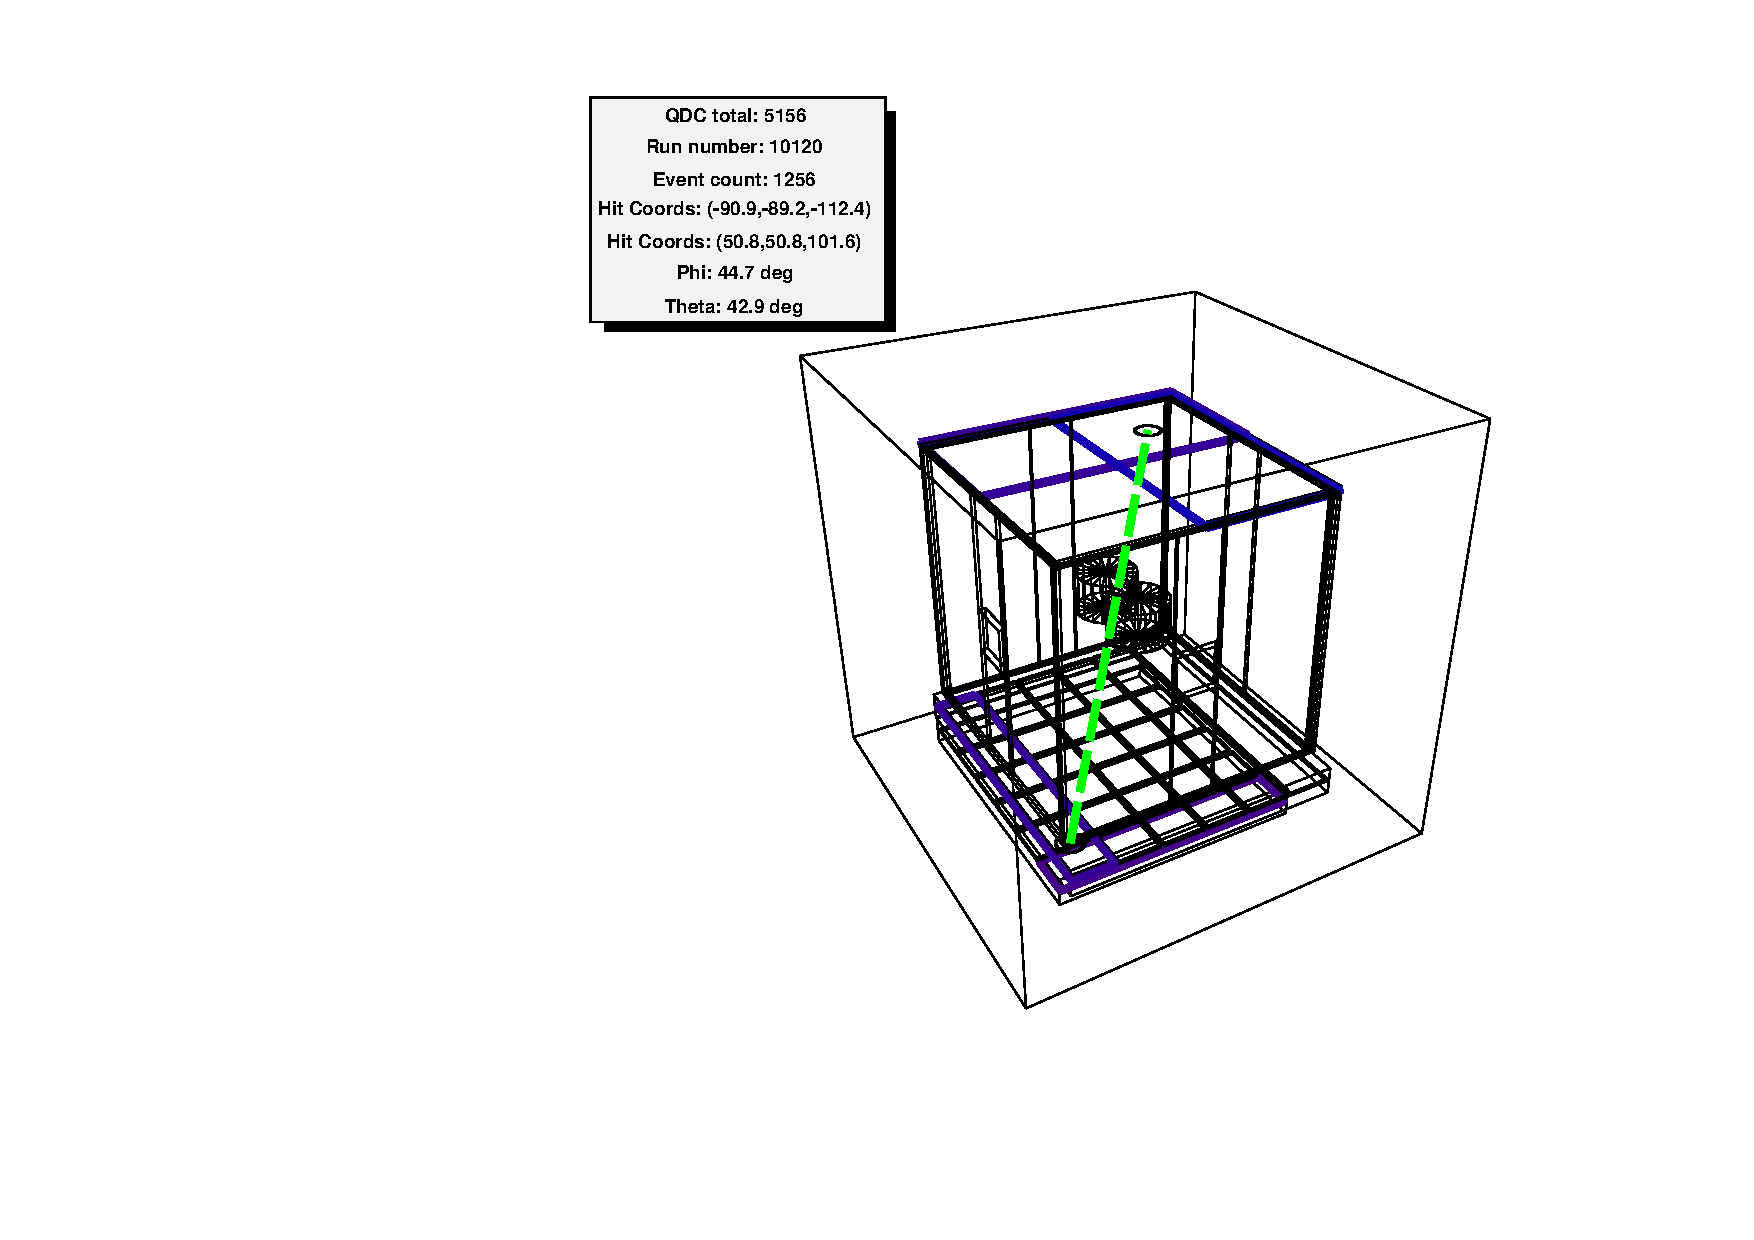
\includegraphics[scale=0.5]{assembly95.pdf}
\end{figure}

\pagebreak

\textbf{Model:} \\
Built using Root's TGeoVolume classes, a mother volume was first drawn, encompassing all other volumes, acting as an outside boundary. The layer volumes were created in the center of the mother volume, and were rotated/translated to their position based on the coordinate system in the figure below. The panels were created inside each layer according to realistic geometry in centimetres, marking where to draw the panels using local coordinates within each layer. The layers were then added to the mother volume as a node to be seen. The cryovats were added in the same manner, using cylinders for detector volume, rather than boxes. An array holding the mother volume coordinate system (rather than local coordinate system) values of the center of each panel was filled as the panels were put in place. This would be used later to determine where to draw the tracks.

\begin{figure}[h]
\centering
\includegraphics[scale=0.3]{Coordinatesystem.pdf}
\end{figure}

Each panel had an associated number according to the figure below:

\begin{figure}[h]
\centering
\includegraphics[scale=0.3]{Panels_2015.pdf}
\end{figure}

Panel hits are kept track by an array of length 32, each number corresponding to it's respective panel, with values being the amount of received QDC per panel. When hit, the panels are lit up different colors according to their QDC on the ranges:

\begin{figure}[h]
\centering
\includegraphics[scale=0.5]{ranges.png}
\end{figure}

A "layer hit" is defined as any two panels hit simultaneously that are on the same side (ex. both northeast panels) and inner/outer. The program loops though the hits, checking for it's "partner panel" (the panel that would make a layer hit), if found, the mother coordinates of the panel are pushed onto a vector holding the location of each layer hit, and a hole is drawn as a thin volume at the mother coordinate location and added to the mother volume as a node. Using Root's TVirtualGeoTrack class, a point is added at the location of the layer hit to be drawn as the path of the particle.

Passed into the function is the number of panels hit, the total QDC value, run number, and event count of each event, which are all added to the text box accompanying the model using Root's TPaveText class. If two panels are hit, the panel numbers are added as well as if the panels are adjacent to each other (this is done by calling a function holding a 32x32 array showing which panels are touching). Also added to the text box is the vector of each layer hit location in three dimensional Cartesian coordinates. Lastly, added to the text box is the phi and theta of the particle's vector path if a particle is drawn (see figure below for definitions of the phi and theta). This is done by using Root's TVector3 class.

\begin{figure}[h]
\centering
\includegraphics[scale=0.3]{freeformthetaphi.pdf}
\end{figure}


\pagebreak

\textbf{Plots:} \\
Declared globally are canvases, each with their own theme, holding groups of plots. They are edited and drawn to their respective canvases with the drawPlots function, and each canvas is printed as a PDF file with the printPlots function. Each plot is described as follows: \\

\begin{figure}[h]
\centering
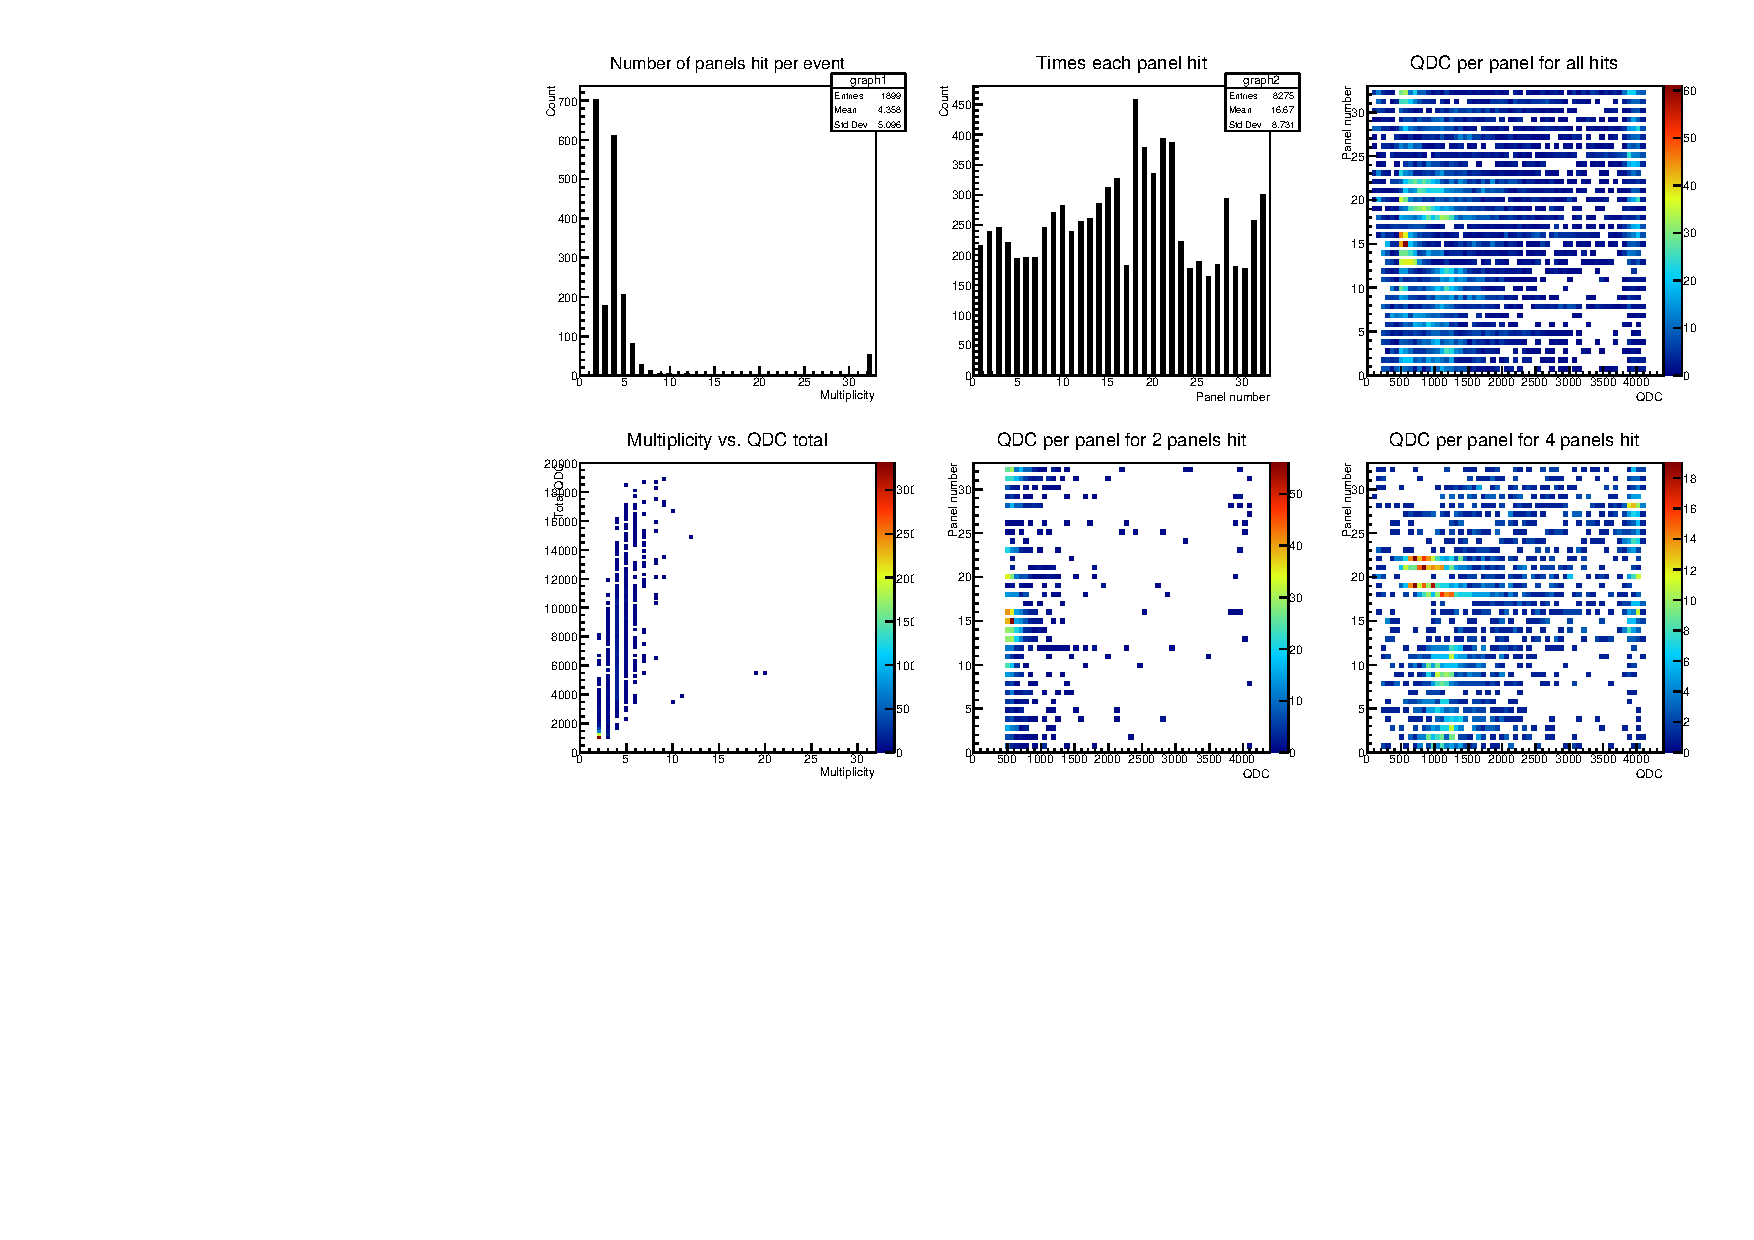
\includegraphics[scale=0.8]{graphs.pdf}
\end{figure}

\textbf{\emph{Number of panels hit per event}:}  \\
This plot describes the total amount of panels hit per event. For each QDC value >0, numberOfPanelsHit is incremented by 1. Filled with the numberOfPanelsHit variable.

\textbf{\emph{Times each panel hit}:} \\
This plot describes how many times each individual panel was hit. Filled by looping through the QDC values and adding any panel above 0 QDC.

\textbf{\emph{QDC per panel for all hits}:} \\
This plot describes how much QDC each panel received per event for every event. Filled by looping through the QDC values and adding any QDC value above 0 QDC.

\textbf{\emph{Multiplicity vs QDC total}:} \\
This plot describes how many panels were hit per event versus the total added QDC of that event. Filled with the numberOfPanelsHit and totalQDC variables.

\textbf{\emph{QDC per panel for 2 panels hit}:} \\
This plot describes the how much QDC each panel received per event for events with only two panels hit. Filled by looping through the QDC values and adding any QDC value and panel number above 0 QDC if it was a two panel event.

\textbf{\emph{QDC per panel for 4 panels hit}:} \\
This plot describes how much QDC each panel received per event for events with only four panels hit. Filled by looping through the QDC values and adding any QDC value and panel number above 0 QDC if it was a four panel event.

\pagebreak
\begin{figure}[h]
\centering
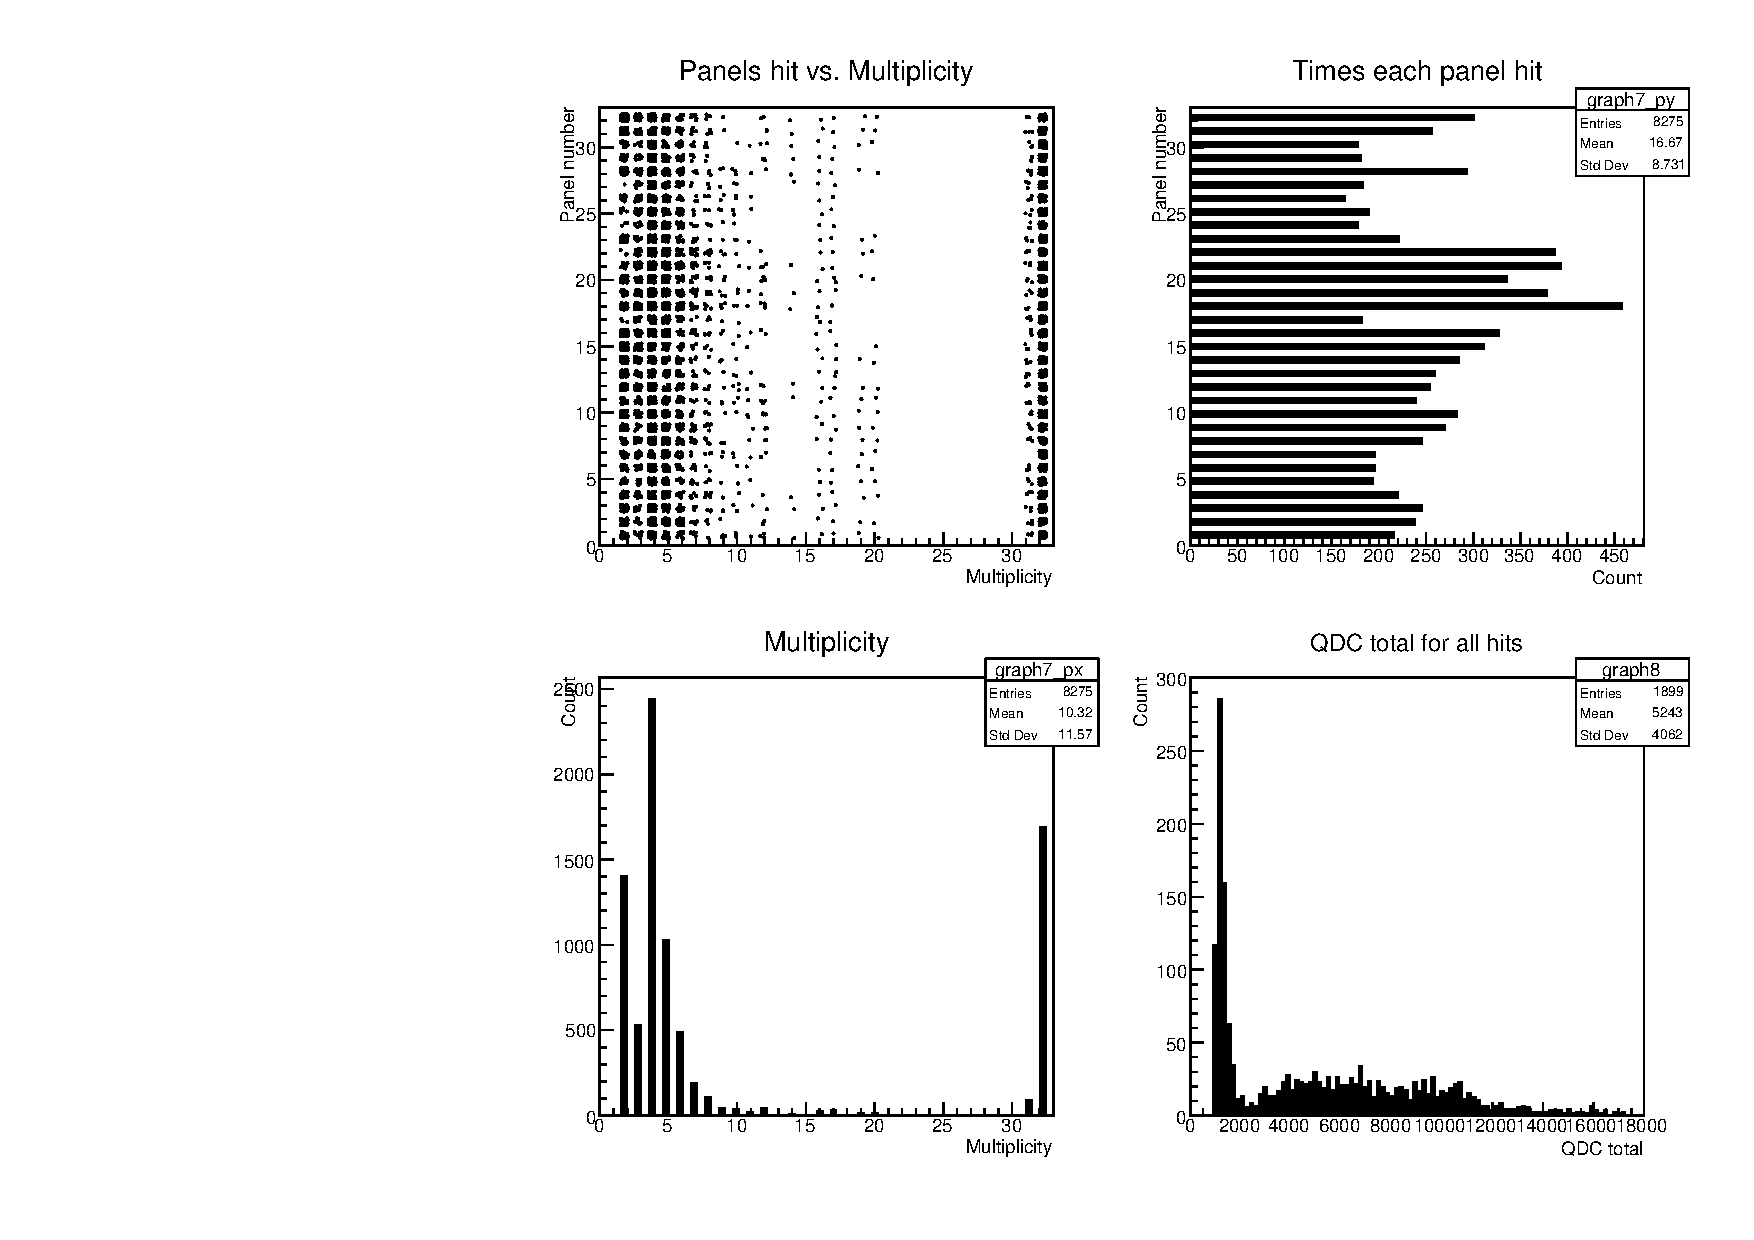
\includegraphics[scale=0.8]{Projections.pdf}
\end{figure}

\textbf{\emph{Panels hit vs Multiplicity}:} \\
This plot describes which panels were hit for each event with n amount of panels hit. Filled by looping through the QDC values and adding any panel above 0 QDC, as well as the numberOfPanelsHit variable.

\textbf{\emph{Times each panel hit}:} \\
A y-axis projection of \emph{Panels hit vs Multiplicity} plot. Describes how many times each panel was hit.

\textbf{\emph{Multiplicity}:} \\
An x-axis projection of \emph{Panels hit vs Multiplicity} plot. Describes how many panels were hit for each event.

\textbf{\emph{QDC total for all hits}:} \\
This plot describes the total added QDC per event for all events. Filled with the totalQDC variable.

\pagebreak
\begin{figure}[h]
\centering
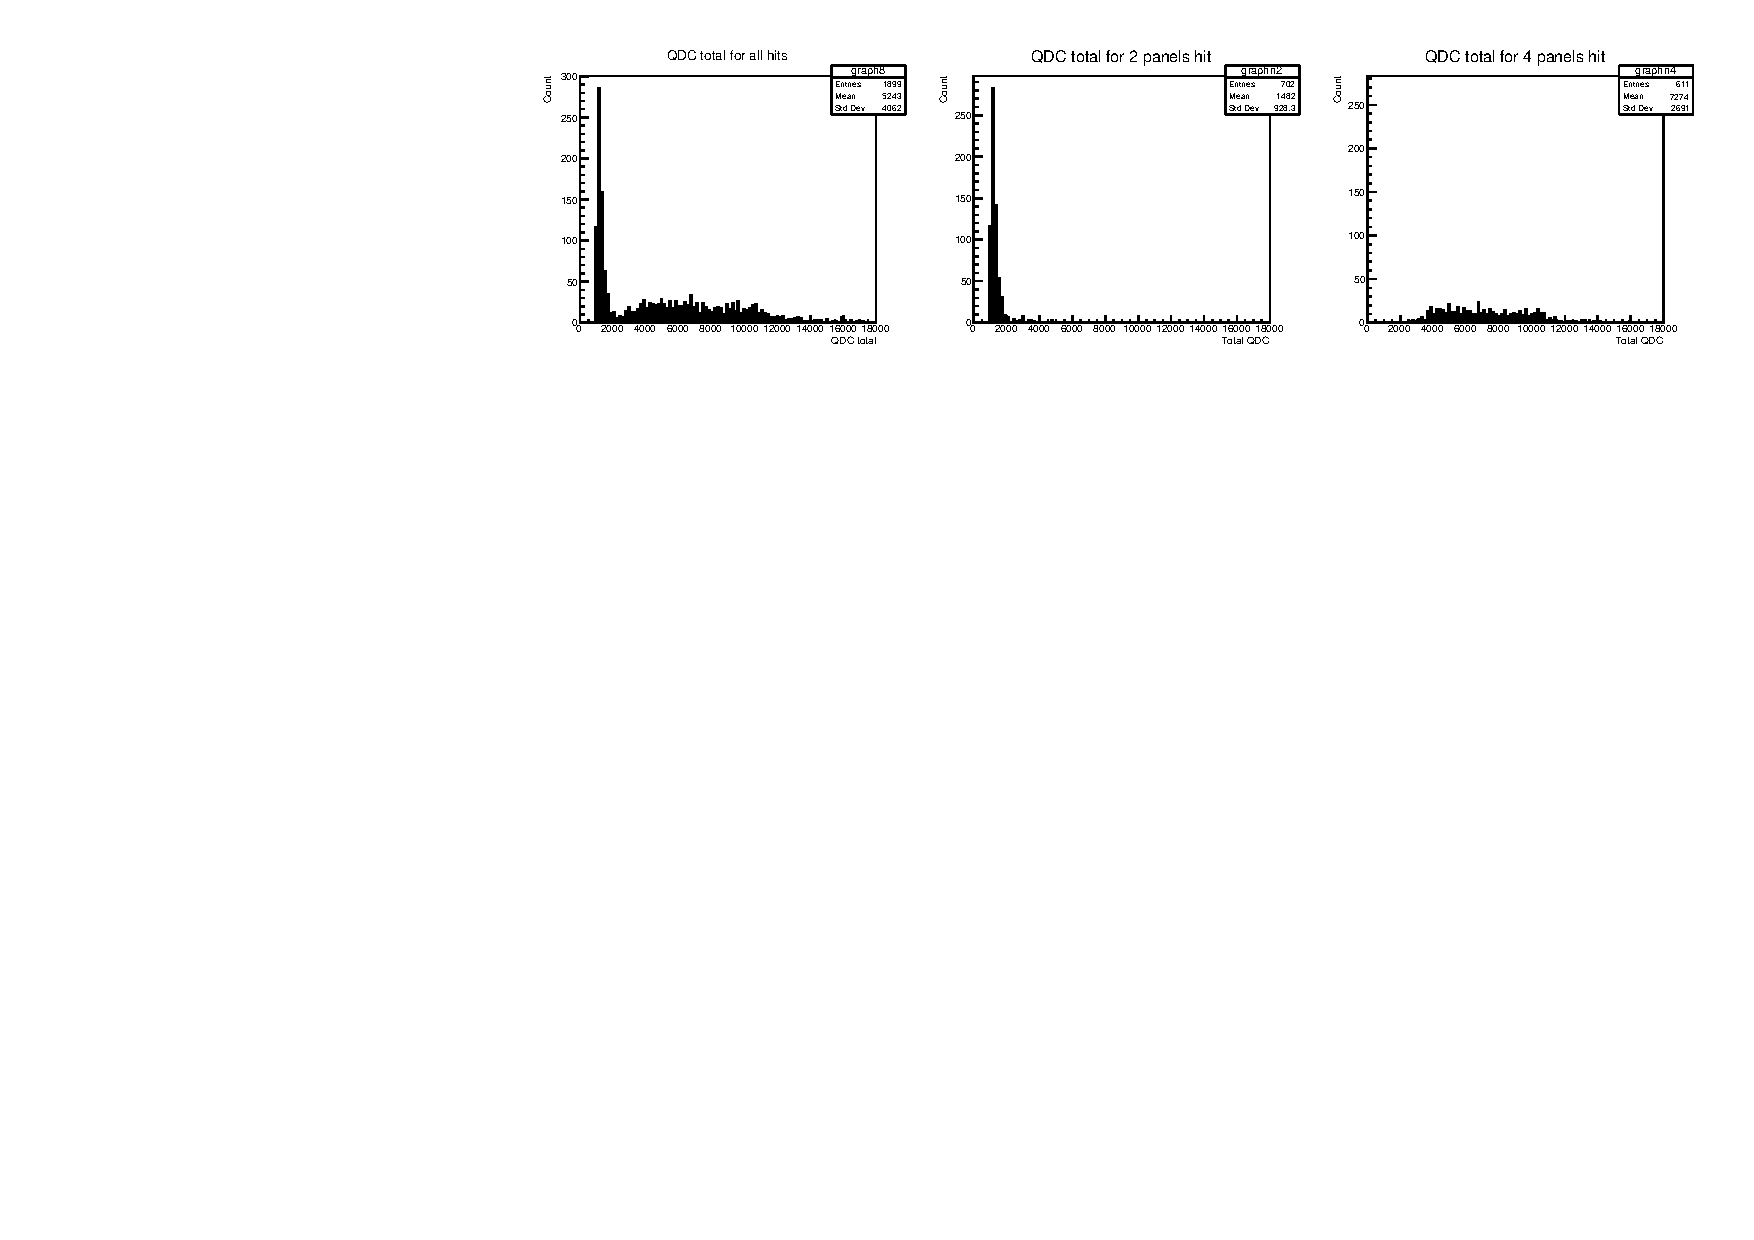
\includegraphics[scale=0.8]{QDCtotal.pdf}
\end{figure}

\textbf{\emph{QDC total for all hits}:} \\
This plot describes the total added QDC per event for all events. Filled with the totalQDC variable.

\textbf{\emph{QDC total for 2 panels hit}:} \\
This plot describes the total added QDC per event for events with only two panels hit.

\textbf{\emph{QDC total for 4 panels hit}:} \\
This plot describes the total added QDC per event for events with only four panels hit.

\pagebreak
\begin{figure}[h]
\centering
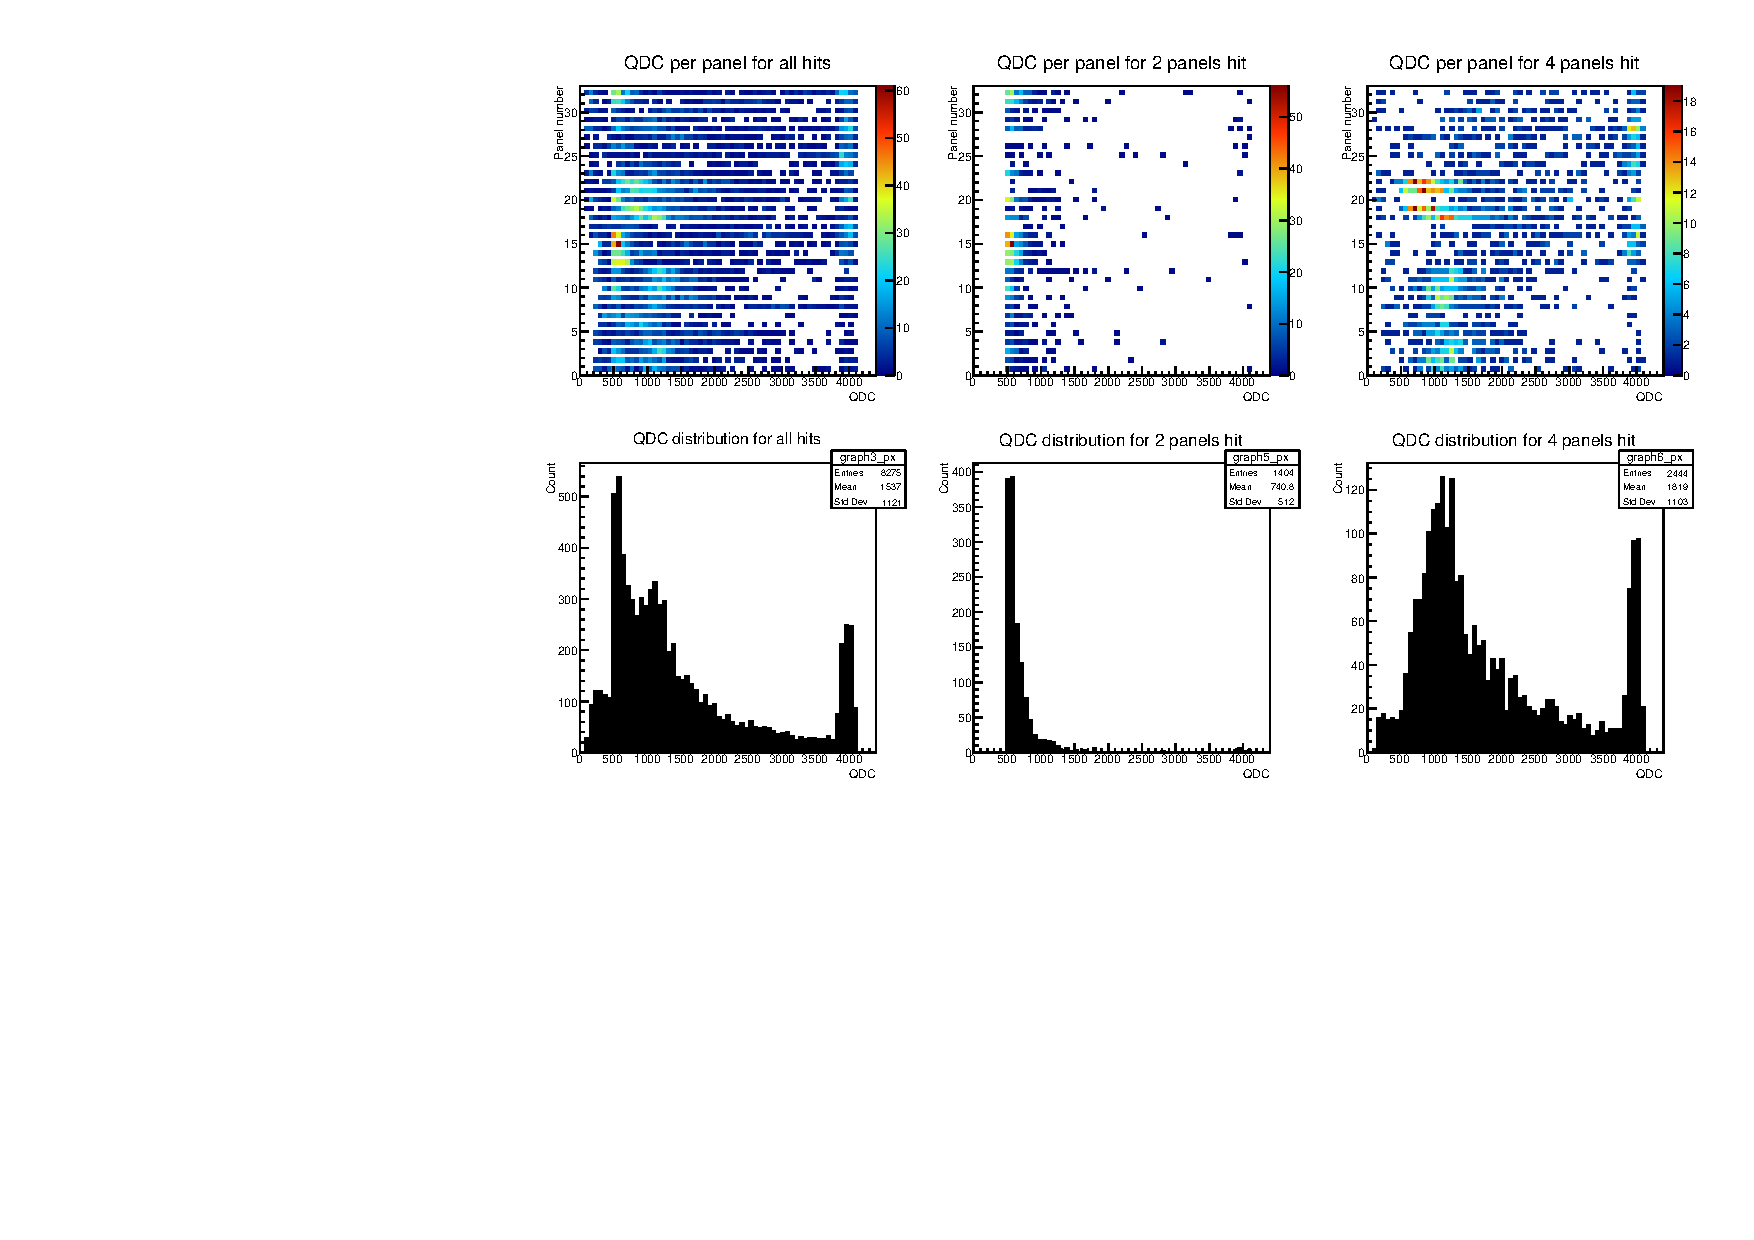
\includegraphics[scale=0.8]{qdcDisplay.pdf}
\end{figure}

\textbf{\emph{QDC per panel for all hits}:} \\
This plot describes how much QDC each panel received per event for every event. Filled by looping through the QDC values and adding any QDC value above 0 QDC.

\textbf{\emph{QDC per panel for 2 panels hit}:} \\
This plot describes the how much QDC each panel received per event for events with only two panels hit. Filled by looping through the QDC values and adding any QDC value and panel number above 0 QDC if it was a two panel event.

\textbf{\emph{QDC per panel for 4 panels hit}:} \\
This plot describes how much QDC each panel received per event for events with only four panels hit. Filled by looping through the QDC values and adding any QDC value and panel number above 0 QDC if it was a four panel event.

\textbf{\emph{QDC distribution for all hits}:} \\
An x-axis projection of \emph{QDC per panel for all hits} plot.

\textbf{\emph{QDC distribution for 2 panels hit}:} \\
An x-axis projection of \emph{QDC per panel for 2 panels hit} plot.

\textbf{\emph{QDC distribution for 4 panels hit}:} \\
An x-axis projection of \emph{QDC per panel for 4 panels hit} plot.

\pagebreak
\begin{figure}[h]
\centering
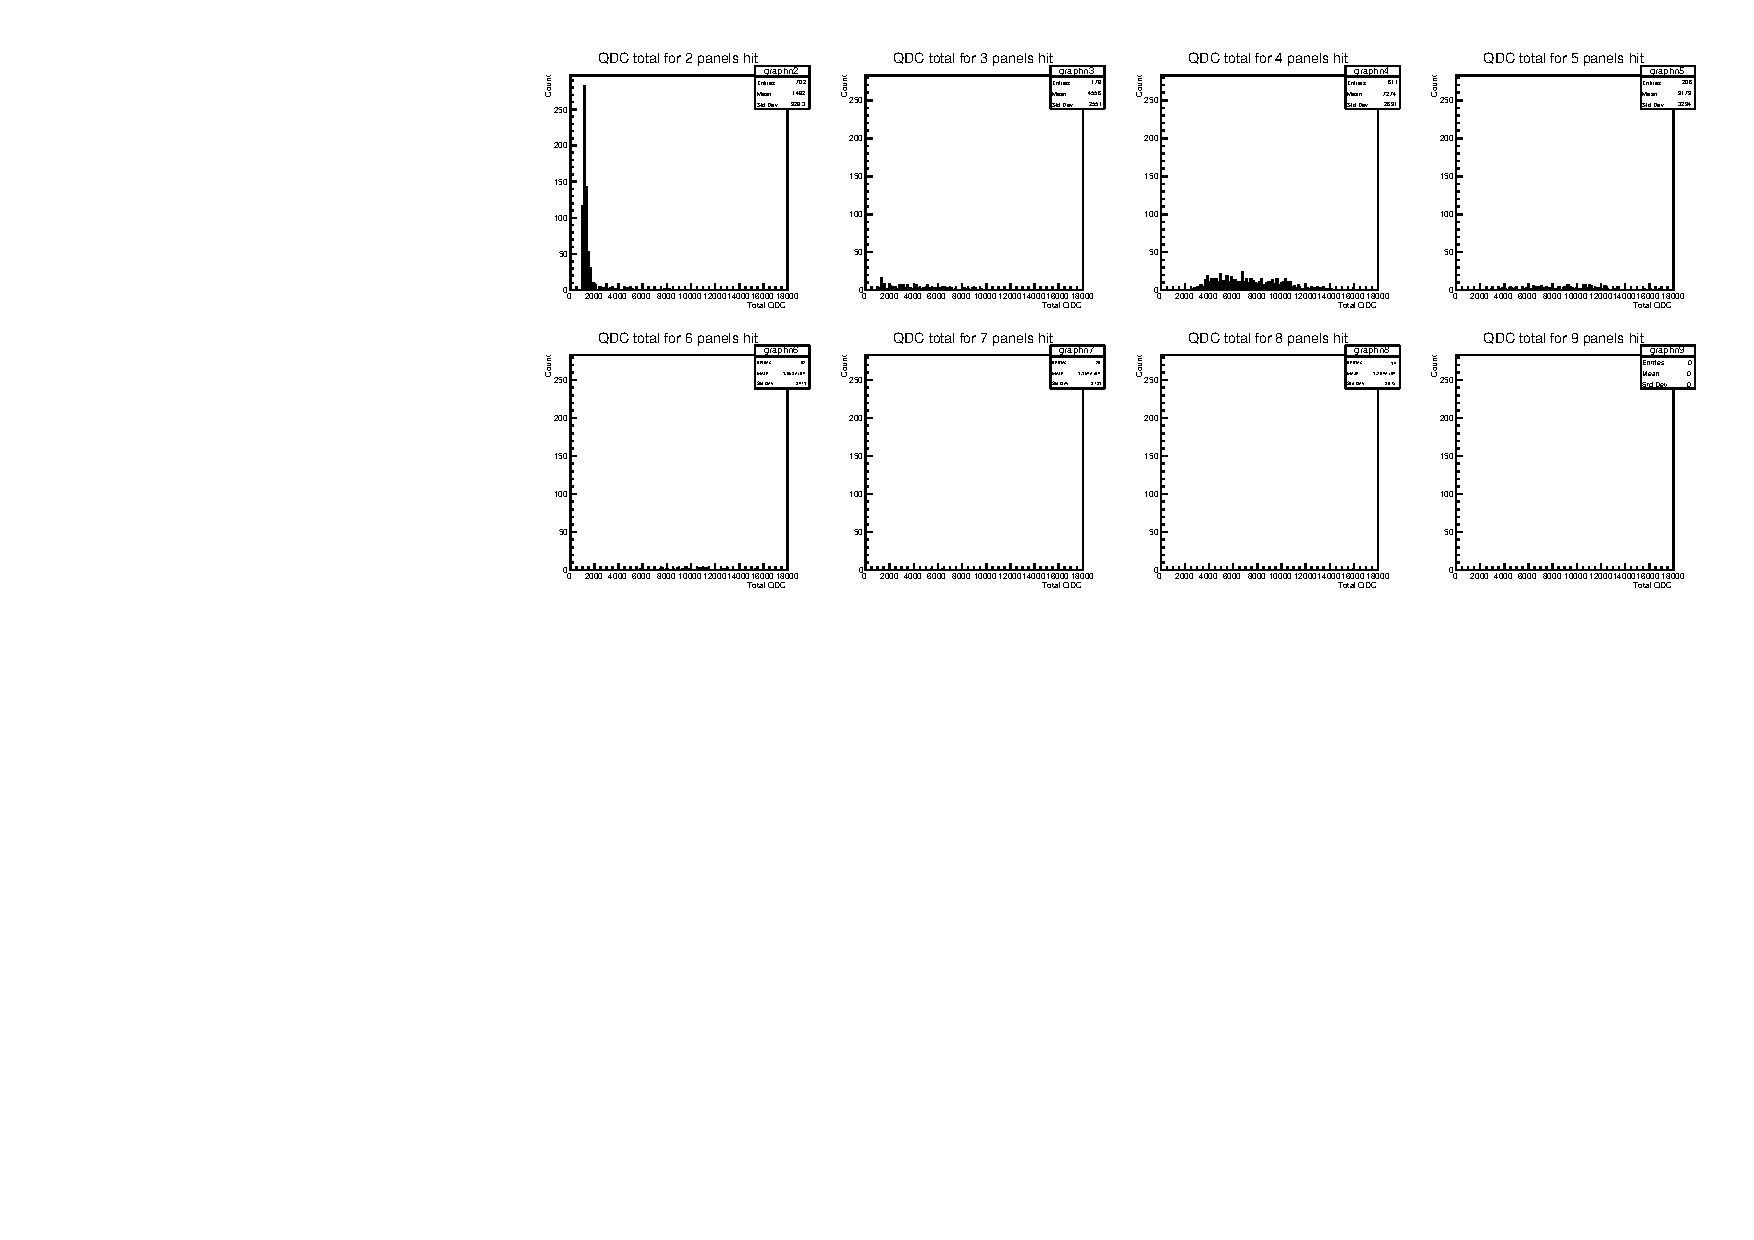
\includegraphics[scale=0.8]{QDCtotaln.pdf}
\end{figure}

\textbf{\emph{QDC total for n panels hit}:} \\
These series of plots describe the total added QDC per event for each event with n panels hit for up to 9 panels hit. Filled by comparing numberOfPanelsHit and adding the totalQDC for each respective hit number.

\pagebreak
\begin{figure}[h]
\centering
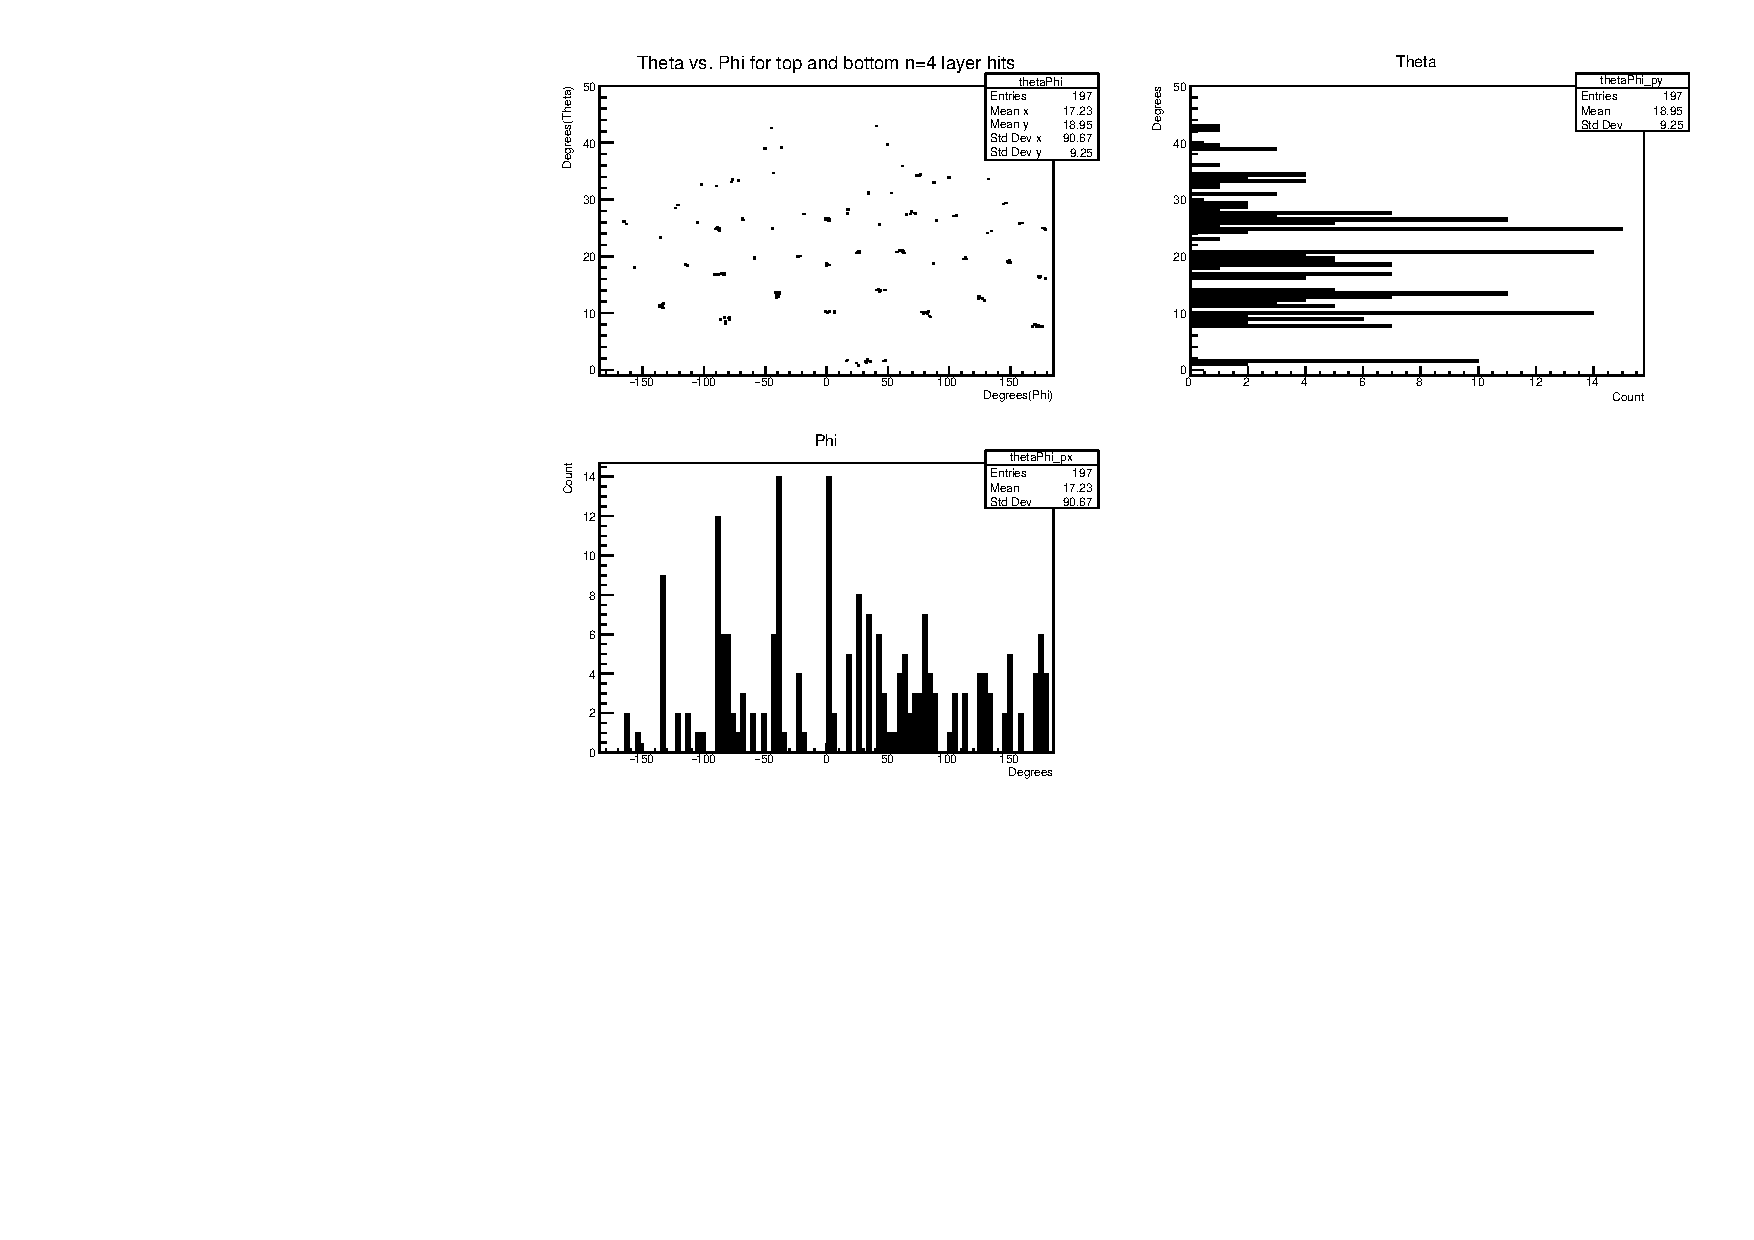
\includegraphics[scale=0.8]{thetaPhi.pdf}
\end{figure}

\textbf{\emph{Theta vs. Phi for top and bottom n=4 layer hits}:} \\
This plot describes the theta and phi spherical angles for the particle's vector for events with 4 panels hit that hit top (inner and outer) and bottom (inner and outer) panels.

\textbf{\emph{Theta}:} \\
A y-axis projection of \emph{Theta vs. Phi for top and bottom n=4 layer hits} plot.

\textbf{\emph{Phi}:} \\
An x-axis projection of \emph{Theta vs. Phi for top and bottom n=4 layer hits} plot.

\pagebreak
\begin{figure}[h]
\centering
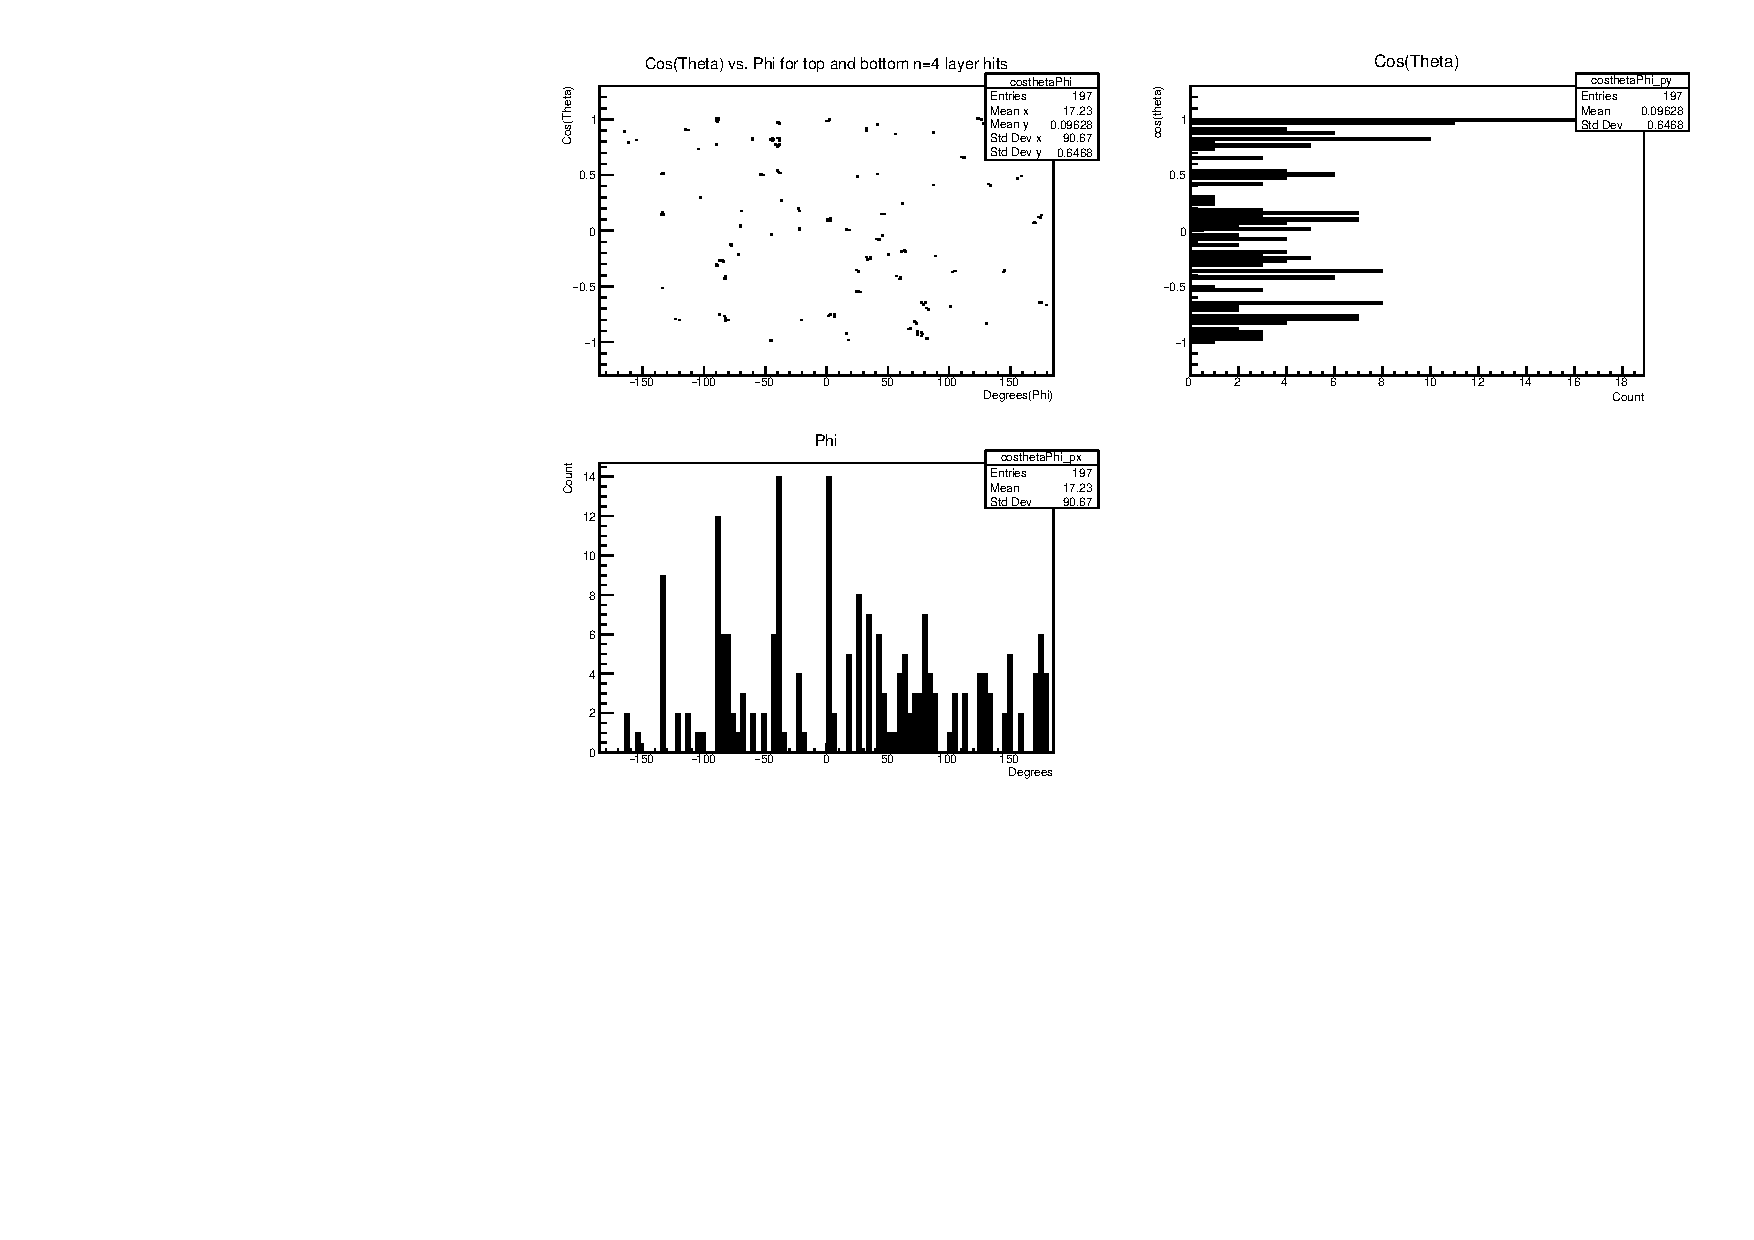
\includegraphics[scale=0.8]{cosThetaPhi.pdf}
\end{figure}

\textbf{costhetaPhi:} "\emph{Cos(Theta) vs. Phi for top and bottom n=4 layer hits}" \\
(costhetaPhi pic) \\
This plot describes the phi and cosine of theta spherical angles for the particle's vector for events with 4 panels hit that hit top (inner and outer) and bottom (inner and outer) panels. 

\textbf{\emph{Cos(Theta)}:} \\
A y-axis projection of \emph{Cos(Theta) vs. Phi for top and bottom n=4 layer hits} plot.

\textbf{\emph{Phi}:} \\
An x-axis projection of \emph{Cos(Theta) vs. Phi for top and bottom n=4 layer hits} plot.

\pagebreak

\textbf{VetoDisplay:} \\
Main:
The input file should be delimited by spaces and in the form: \\
\texttt{runNumber entry eventCount scalerTime QDCvaluePanel1 QDCvaluePanel2 ... QDCvaluePanel32} \\
ex. \\
\texttt{9959 14359 1037 3003.45 0 0 0 0 1283 0 0 1407 0 0 0 0 0 0 0 0 0 1556 0 0 0 968 0 0 0 0 0 0 0 0 0 0 } \\
The program opens the input file and loops through each event. For an individual event, if the QDC value (stored in an array of size 32) is greater than 0, numberOfPanelsHit variable is incremented by 1, and the value is added to the totalQDC variable. Any missing panels (if less than 32 panels were given) are filled with a value of 0 QDC. With the necessary variables, drawEvent and fillPlots are called to draw the wireframe model and fill each plot with the event data. 

After the program has looped through all the events, a heatmap of all the hits are drawn. This is accomplished by summing all the QDC values per panel for every event, multiplying it by a scale factor, and calling drawEvent one last time with the scaled values. The scale factor is denoted by: \\
\texttt{scaleFactor = (MaxColorValue - MinColorValue) / (maxSumValue - minSumValue)} \\
The heatmap is created as a PDF and the drawPlots and printPlots functions are called to generate and print the plots as a PDF file.

The 0-31 panel numbering format is used in all programming aspects, but is displayed on the text box and plots in the 1-32 format, to mitigate confusion.

\textbf{Functions:} \\
	The isNextTo function is used for the text box to find if two panels are adjacent. A 32x32 matrix cooresponds to each panel, getting a 1 if the panel is next to it, and a 0 if it is not. For example, if panel 3 is next to panel 20(on the 1-32 scale), panelTable[2][19] should return a 1. 

The isLayerHit function is used for checking if a layer partner exists. A 32x32 matrix similar to the isNextTo fuction returns a 1 provided the second panel is a layer partner. The bottom and upper panels have more than one layer partner, whereas the sides do not.

The hitLocation function is used for getting the location of a layer hit in the mother coordinate system. The function pushes either the x value or y value of a panel onto a vector depending if it is the top layer or not.

The hitFinder function is used to get a 3-D rotatable model of an individual event. The function opens with Root's TApplication classes. A canvas is drawn after the run number and event count is found, and is automatically put on the TApplication window. Finally, the application is run. To access the hitFinder function, run the executable with ./VetoDisplay runNumber eventCount. 

\pagebreak


\end{document}